%# -*- coding: utf-8-unix -*-

\chapter{评估测试}
\label{chap:evaluation}

评估测试部分主要涉及Appetizer客户端SDK在Android设备上的影响,因为对于使用Appetizer客户端SDK的开发者来说,他们关心的主要问题是SDK对于原来Android应用程序的性能影响、空间占用应用等,Appetizer服务端是隐藏的黑盒。
因此本篇文章介绍的Appetizer整套系统中,和同类产品相比核心竞争力之一是Appetizer客户端SDK的各项指标。

\section{功能对比}

功能列表


\section{SDK空间占用对比}

对于做用户数据收集的Android SDK,集成到Android应用程序占用的额外空间同样是一个重要指标。因为作为第三方工具库,本身占用空间的增大会造成所有集成该工具库的占用空间变大,影响范围较广,因此第三方工具库的占用空间越小越好。

表\ref{tab:SDK_size}展示的是Appetizer和同类Android SDK占用空间的数据,表中列举的产品中ACRA的功能覆盖面最小,本文介绍的Appetizer客户端SDK在功能覆盖上是ACRA的超集,减少部分崩溃信息可定制化的功能,增加了注入用户会话信息、Andorid程序未响应侦测等功能,但是占用空间更小。其他产品在功能上和Appetizer相比各有千秋,占用空间都远超Appetizer客户端SDK。

图\ref{fig:SDK_size}展现的是Appetizer和同类Android SDK占用空间倒数的柱状图,可以等价于各个产品在占用空间上的得分,更直观的展现了Appetizer客户端SDK轻量级的优势。

\begin{table}[!hpb]
	\centering
	\bicaption[tab:SDK_size]{指向一个表格的表目录索引}{产品SDK占用空间表}{Table}{Product SDK size table}
	\begin{tabular}{@{}llr@{}} \toprule
		Product & Version &Size \\ \midrule
		Appetizer &v0.1& 71 kB \\
		Umeng&v6.0.1& 301 kB \\
		TalkingData&v2.2.25& 386 kB \\
		ACRA&v4.9.0& 152 kB \\
		Flurry Analytics&v6.3.1& 260 kB \\ \bottomrule
	\end{tabular}
\end{table}

\begin{figure}[!htp]
	\centering
	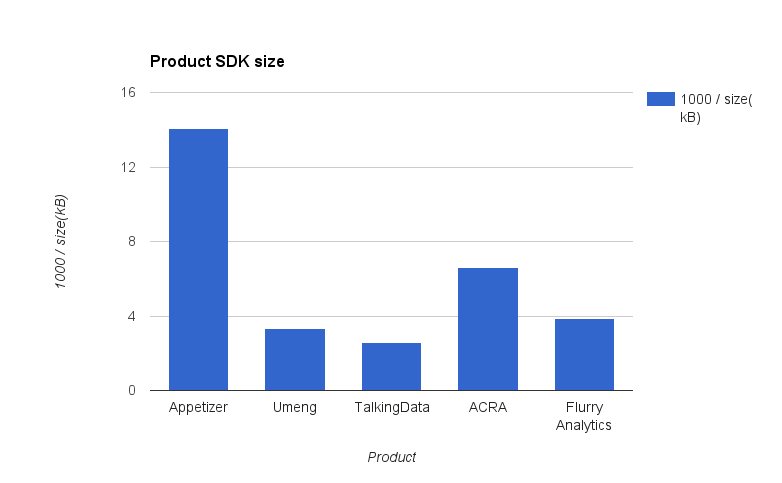
\includegraphics[width=0.9\textwidth]{SDK_size.png}
	\bicaption[fig:SDK_size]{这里将出现在插图索引中}{产品SDK占用空间}{Fig}{Product SDK size}
\end{figure}

\section{性能对比}





\section{本章小节}

